\documentclass[10pt]{beamer}
\hypersetup{pdfpagemode=FullScreen}
\usepackage[spanish, es-tabla]{babel}  
\selectlanguage{spanish}
\usepackage[utf8]{inputenc}

% ----- Tiene que ver con el tema de la presentación -----------------------------
\usetheme[progressbar=frametitle]{metropolis}
\usepackage{appendixnumberbeamer}
\usepackage{booktabs}
\usepackage[scale=2]{ccicons}
\usepackage{pgfplots}
\usepgfplotslibrary{dateplot}
\usepackage{xspace}
\newcommand{\themename}{\textbf{\textsc{metropolis}}\xspace}
%---------------------------------------------------------------------------------
\usepackage{minted}    % Formato de python
\usepackage{xcolor}
\usepackage{gensymb} % Para generar ciertos símbolos en modo texto.

\title{Taller de Python}
\subtitle{Clase II}
% \date{\today}
\date{}
\author{Comisión de Talleres}
\institute{Centro de Estudiantes Tecnológicos}
%\titlegraphic{\hfill
\includegraphics[height=1.5cm]{FondoACET}}

\begin{document}

\maketitle

\begin{frame}{Tabla de contenidos}
  \setbeamertemplate{section in toc}[sections numbered]
  \tableofcontents[hideallsubsections]
\end{frame}
\section{Introducción}
\begin{frame}{Paquetes}
	Un \alert{paquete} puede ser interpretado como un directorio de \emph{scripts}.
	
	\vspace{1em}
	
	Cada \emph{script} es un \alert{módulo}, donde se especifican funciones, métodos y tipos.
	
    \vspace{1em}

	\textbf{No todos los paquetes disponibles están instalados por defecto}, pero anaconda nos ofrece una manera muy sencilla de instalar  aquellos paquetes que podamos necesitar.
\end{frame}
\section{Numpy}
\begin{frame}{¿De qué se trata?}
\textbf{NumPy} es un paquete fundamental para la programación científica que proporciona un objeto tipo \alert{array} para almacenar datos de forma eficiente y una serie de funciones para operar y manipular esos datos. 

Los arrays proporcionados por NumPy son más eficientes que las listas y nos permiten realizar diferentes cálculos.

Para conocer más de lo que ofrece esta librería ir a:

\begin{center}
	\url{http://www.numpy.org/}
\end{center}
\end{frame}

\begin{frame}[fragile]{Importando}
Para utilizar esta librería es necesario importarla.
\begin{minted}[bgcolor=brown!10!white]{python}
import numpy
import numpy as np 
from numpy import * 
\end{minted}
\begin{center}
	¿Da lo mismo ocupar cualquiera de estas opciones?
\end{center}
\end{frame}


\begin{frame}[fragile]{¿Qué nos ofrece?}
Por medio del comando \alert{dir()} es posible saber qué ofrece este paquete.
\begin{minted}[bgcolor=brown!10!white]{python}
dir(numpy) 
\end{minted}
Para saber un poco más acerca de algún elemento en particular:
\begin{minted}[bgcolor=brown!10!white]{python}
help(numpy.array)
\end{minted}
\end{frame}

\begin{frame}[fragile]{numpy.array()}
	\textbf{Numpy arrays} son estructuras muy similares a las listas, pero pueden contener un solo tipo de datos.
	\begin{center}
		¿Qué ocurre cuando un array está formado por datos de diferentes tipos?
	\end{center}
	\begin{minted}[bgcolor=brown!10!white]{python}
np_array1 = np.array([1,2,False])
np_array1.dtype 
	\end{minted}
	
	\only<2>{\begin{center}
			True y False se transforman en 1 y 0, respectivamente
	\end{center}}
\end{frame}

\begin{frame}[fragile]{numpy.array()}
	Que los datos sean de un único tipo permite llevar a cabo cálculos de forma muy eficiente. Sin embargo, es importante hacer notar también que existen otras diferencias con las listas. 
	
	\begin{minted}[bgcolor=brown!10!white]{python}
>>> np_array1 = np.array([1, 2, False])
>>> np_array2 = np.array([True, 3, 4])
>>> np_array3 = np_array1 + np_array2
>>> np_array3
array([2, 5, 4])

>>> [1, 2, False] + [True, 3, 4]
[1, 2, False, True, 3, 4]
	\end{minted}
\end{frame}

\section{Matplotlib}
\begin{frame}{Matplotlib}
	Matplotlib es una librería para realizar gráficos en 2D capaz de generar figuras de excelente calidad.
	
	El siguiente enlace nos lleva a su documentación, donde es posible encontrar gran variedad de ejemplos con sus respectivos códigos.
	
	\begin{center}
		\url{http://matplotlib.org/}
	\end{center}  
\end{frame}

\begin{frame}[fragile]{Matplotlib.pyplot}
	Lo que ocuparemos es un subpaquete de matplotlib llamado \alert{pyplot}, y lo importaremos de la siguiente manera:
	\vspace{1em}
	\begin{minted}[bgcolor=brown!10!white]{python}
import matplotlib.pyplot as plt
	\end{minted}
	Importando numpy como np y matplotlib.pyplot como plt
	\begin{minted}[bgcolor=brown!10!white]{python}
t = np.linspace(1,10,500)
y = np.sin(2*t)

plt.plot(t,y)
plt.show()
	\end{minted}
\end{frame}

\begin{frame}
	\begin{figure}
		\scalebox{0.55}{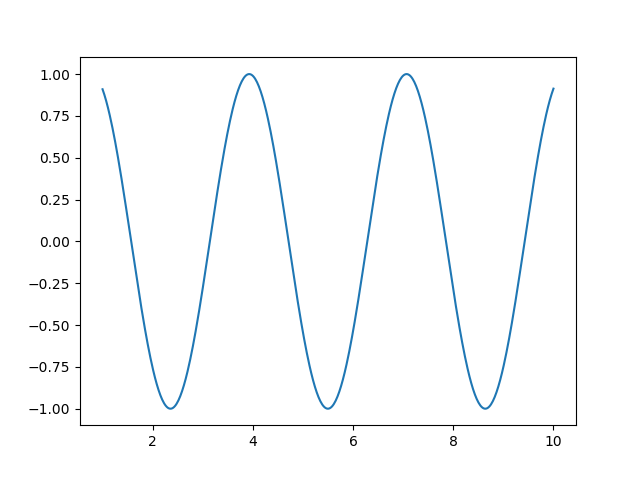
\includegraphics{figure_sin}}
		\caption{Gráfico de la función $y = sin(2t)$}
	\end{figure}
\end{frame}

\begin{frame}[fragile]{Ejemplo}
	Si tenemos datos en un archivo de texto, numpy nos ofrece la posibilidad de importarlos con el siguiente comando. Los datos son asignados a nuestra variable \alert{Escalon}.
	\begin{minted}[bgcolor=brown!10!white]{python}
Escalon = np.loadtxt('Sis_subamortiguado.txt', 
		delimiter=',')
	\end{minted}

	La primera columna son valores de tiempo y la segunda el valor de cambio de una variable bajo estudio.
	
	\begin{minted}[bgcolor=brown!10!white]{python}
plt.plot (Escalon[0], Escalon[1])
plt.show()
	\end{minted}
\end{frame}

\begin{frame}
	\begin{figure}
		\scalebox{0.55}{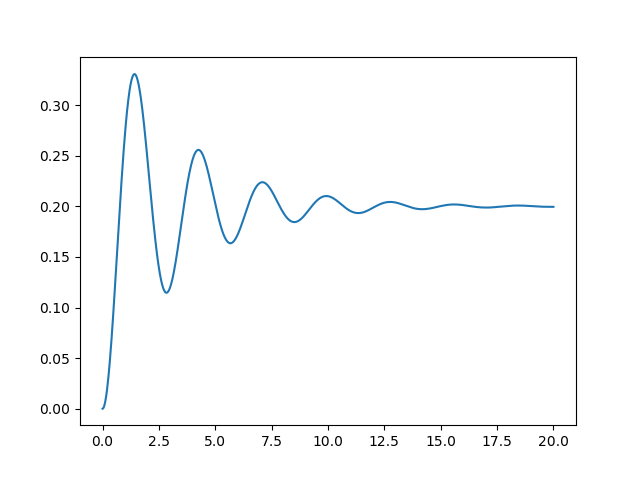
\includegraphics{figure_sub}}
		\caption{Sistema subamortiguado}
	\end{figure}
\end{frame}

\begin{frame}[fragile]{Personalización}
	El fragmento de código mostrado a continuación nos enseña como:
	\begin{itemize}
		\item variar el grosor del trazo con \alert{linewidth},
		\item añadir etiquetas a los ejes con \alert{xlabel} y \alert{ylabel},
		\item añadir un título al gráfico con \alert{title}, y
		\item modificar los límites de los ejes con \alert{axis}.
	\end{itemize}
	\begin{minted}[bgcolor=brown!10!white]{python}
plt.plot(Escalon[0], Escalon[1], linewidth=2.0)
plt.xlabel('Tiempo')
plt.ylabel('Respuesta')
plt.title('Sistema subamortiguado')
plt.axis([0, 20, 0, 0.35])
	\end{minted}
\end{frame}

\begin{frame}
	\begin{figure}
		\scalebox{0.55}{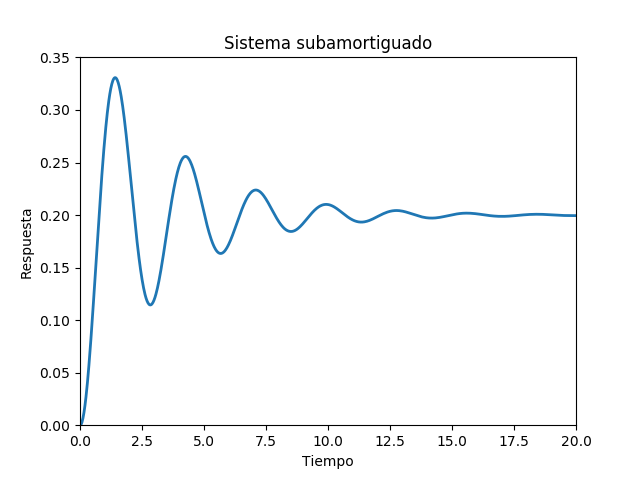
\includegraphics{figure_sub2}}
		\caption{Gráfico con títulos, etiquetas y escala modificada.}
	\end{figure}
\end{frame}

\begin{frame}[fragile]{Personalización}

La función \textbf{plot} grafica líneas rectas y le basta con dos puntos, en el fragmento de código se traza una recta horizontal que pasa por los puntos (0, 0.20) y (20,0.20).
\vspace{1em}

Es posible incorporar leyendas para una descripción más detallada, modificar el tipo de trazo y el color.

	\begin{minted}[bgcolor=brown!10!white]{python}
plt.plot((0,20),(0.20,0.20), '--k', 
label='Estado estacionario')

plt.legend(loc='best')
	\end{minted}
\end{frame}

\begin{frame}
	\begin{figure}
		\scalebox{0.55}{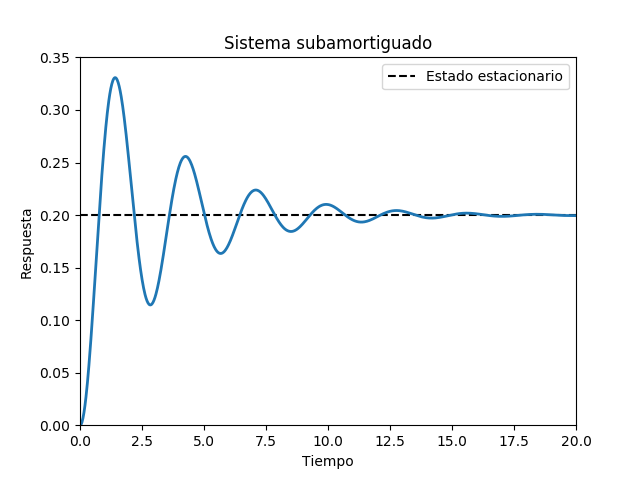
\includegraphics{figure_sub3}}
		\caption{Gráfico con línea adicional y leyenda.}
	\end{figure}
\end{frame}

\begin{frame}[fragile]{Personalización}

Se puede incorporar texto en una determinada posición con la función \alert{text}. En el fragmento de código se muestra como modificar la fuente por medio de un diccionario.

	\begin{minted}[bgcolor=brown!10!white]{python}
font = {'family': 'serif',
'color':  'darkred',
'weight': 'normal',
'size': 12,
}

plt.text(2, 0.05, 'Es posible incorporar texto.',
		 fontdict=font)
	\end{minted}
\end{frame}

\begin{frame}
	\begin{figure}
		\scalebox{0.55}{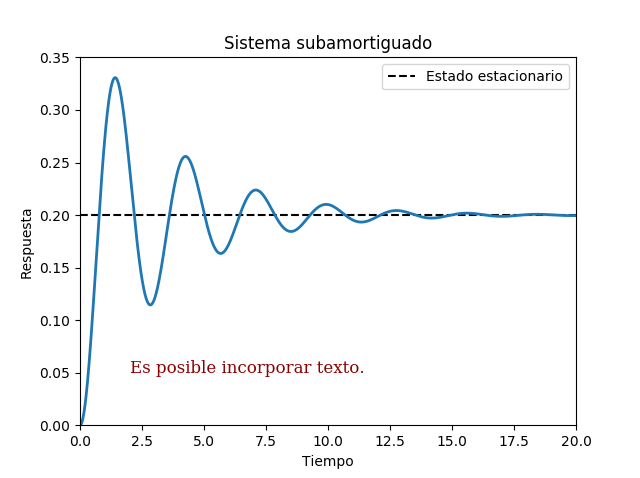
\includegraphics{figure_sub4}}
		\caption{Gráfico con texto aclaratorio.}
	\end{figure}
\end{frame}

\begin{frame}[standout]
	¿Preguntas?
\end{frame}

\appendix

\begin{frame}{Enlaces de interés}
	\begin{itemize}
		\item \alert{Comunidad Python Argentina}\\ \url{http://www.python.org.ar}
		\item \alert{AeroPython}\\ \url{https://github.com/AeroPython}
		\item \alert{Tutorialspoint}\\ \url{https://www.tutorialspoint.com/index.htm}
		\item \alert{Byte of Python}\\ \url{https://python.swaroopch.com/control_flow.html}
		\item \alert{Python programming}\\ \url{https://pythonprogramming.net}
	\end{itemize}
\end{frame}
\section{Fin de la segunda clase}
\end{document}
